
\subsection{Definition}

\textbf{Dynamic programming} is a method for solving a complex problem by breaking it down 
into a collection of simpler subproblems, \textbf{solving each of those subproblems just once, 
and storing their solutions in memory}. The next time the same subproblem occurs, instead of 
recomputing its solution, one simply looks up the previously computed solution, thereby 
\textbf{saving computation time at the expense of storage space}.

\subsection{Solving the knapsack problem with DP}

\subsubsection{The knapsack problem}

The knapsack problem is specified as follow : Given a set of item I, each item i being 
associated with a given value $(V_i)$ and weight $(W_i)$. Maximize the value of 
selected items. 

\begin{center}
\Large{$\sum_{i \in I} v_i x_i$}
\end{center}

Under constraint that the total capacity cannot exceed a given maximal capacity C 
and that an item cannot be partially selected. \newline

\begin{center}
\Large{$\sum_{i \in I} w_i x_i \le C$}

\vspace{3 mm}
\Large{$x_i \in \{0,1\}$}
\end{center}

Note that Knapsack is an NP-Complete problem as it can be used
to find a solution to the subset sum problem, which is NP-complete.

\begin{figure}[!ht]
	\centering
	\begin{framed}
	Given a set of natural number and a capacity K. 
	Find a subset S such that :\newline
	\Large{$\sum_{i \in S} c_i = K$}
	\end{framed}
	\caption{Subset sum problem}
\end{figure}
\FloatBarrier

\subsubsection{Breaking knapsack in subproblems}

Let us refer to the optimal objective of the problem with capacity k and
items \{1,…,j\} $\in$ I as O(k,j). We can easily notice that :

\[ O(k,0) = 0 \text{\footnotemark}\]
\[ O(k,j) = \begin{cases} 
      max(O(k,j-1) , vj +O(k-wj,j-1))\text{\footnotemark} & if \quad w_j \leq k \\
      O(k,j-1) & otherwise
   \end{cases}
\]
\footnotetext{As their are no elements to choose from}
\footnotetext{Bellman's equations}

\begin{figure}[!ht]
    \centering
    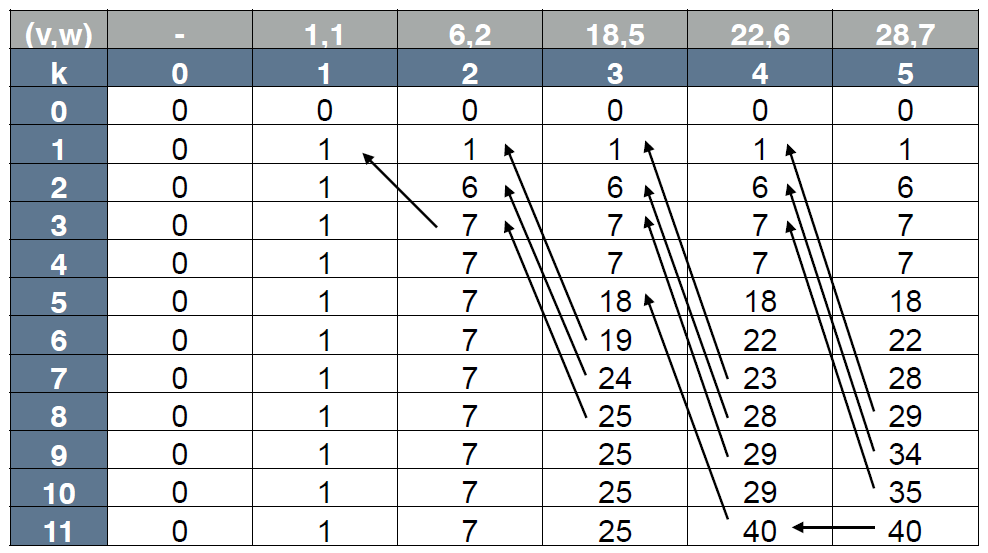
\includegraphics[width=0.7\linewidth]{KnapsackDP.png}
    \caption{Basic Knapsack resolution example (no cache)}
    \label{fig:Knapsack_example}
\end{figure}
\FloatBarrier

\subsubsection{DP algorithm for knapsack in $\theta$(Cn)}

We can thus implement an algorithm finding O(C,n), using the previously 
stated formula. As calculating O(C,n) may imply many sub problem recalculation,
we will cache the results of each sub problem in a map.

\begin{figure}[!ht]
    \centering
    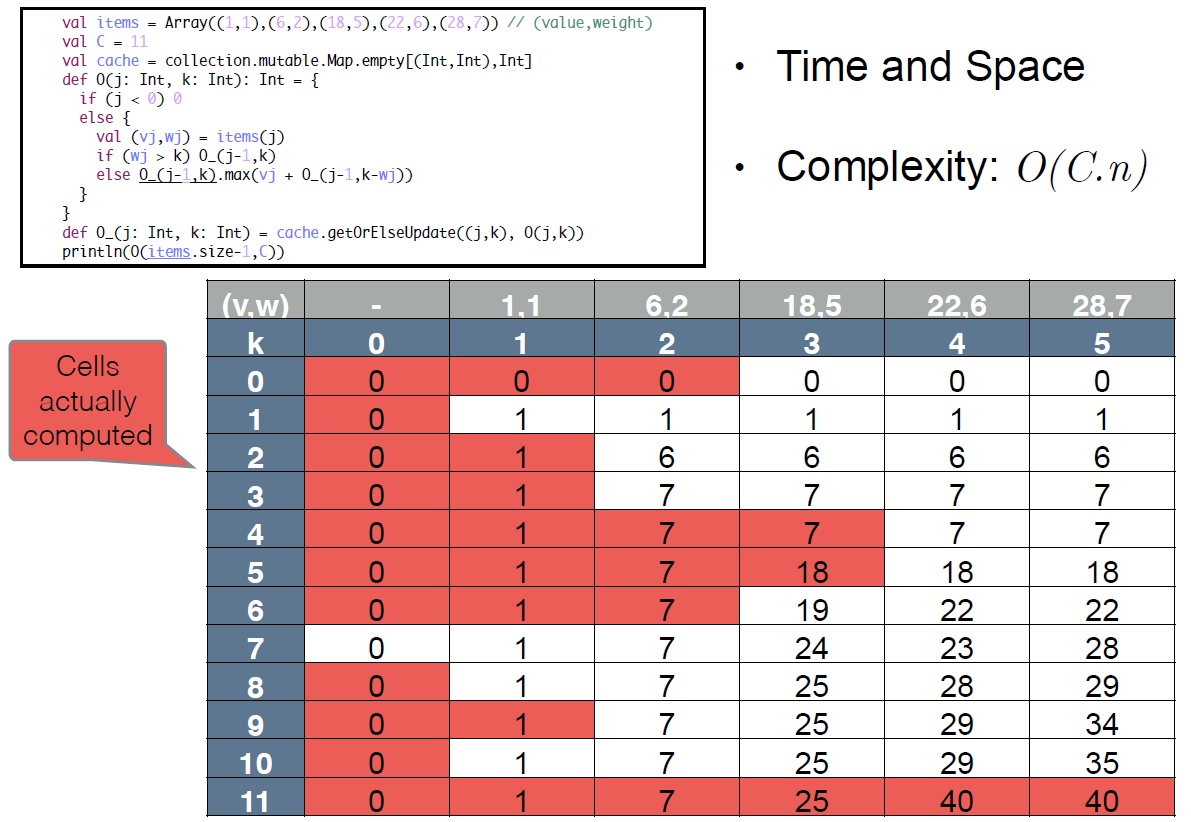
\includegraphics[width=\linewidth]{KnapsackDPAlgo1.png}
    \caption{Knapsack DP algorithm in scala}
    \label{fig:Knapsack_example}
\end{figure}
\FloatBarrier

\textbf{Although this algorithm works, his time/space complexity is not polynomial} 
as log(C) bits are necessary to represent C. The complexity is thus exponential
relatively to the input size. This algorithm is thus \textbf{weakly NP-Complete} or 
\textbf{pseudo-polynomial}\footnote{a numeric algorithm runs in pseudo-polynomial time if its running time is polynomial in the numeric value of the input, but is exponential in the length of the input – the number of bits required to represent it.} as it is roughly polynomial for small values of C while computing larger value is much more expensive\footnote{Not all NP-Complete algorithm are pseudo polynomial ! Like the 
traveling salesman problem (TSP), for example.}.

\subsubsection{DP algorithm for knapsack in $\theta$(Vn)}

Using a similar logic, it is also possible to define an algorithm which run in 
$\theta$(Vn) to compute knapsacks. For this, we must first define V as :\newline

\begin{center}
\Large{$V = \sum_{i \in I} v_i$}
\end{center}

And then redefine O(k,j) as O(w,j), the optimal weight using only items \{1,...,j\}. The equation will thus change as follow :

\[ O(0,j) = O(w,0) = 0 \text{\footnotemark} \]
\[ O(w,j) = \begin{cases}
      min(O(w,j-1), wi + O(w-v_j,j-1)) & if \quad v_j \leq p \\
      O(w,j-1) & otherwise
   \end{cases}
\]
\footnotetext{As $w_i > 0$ for all $i \in I$ and as we cannot have w > 0 with 
an empty set.}

\begin{figure}[!ht]
    \centering
    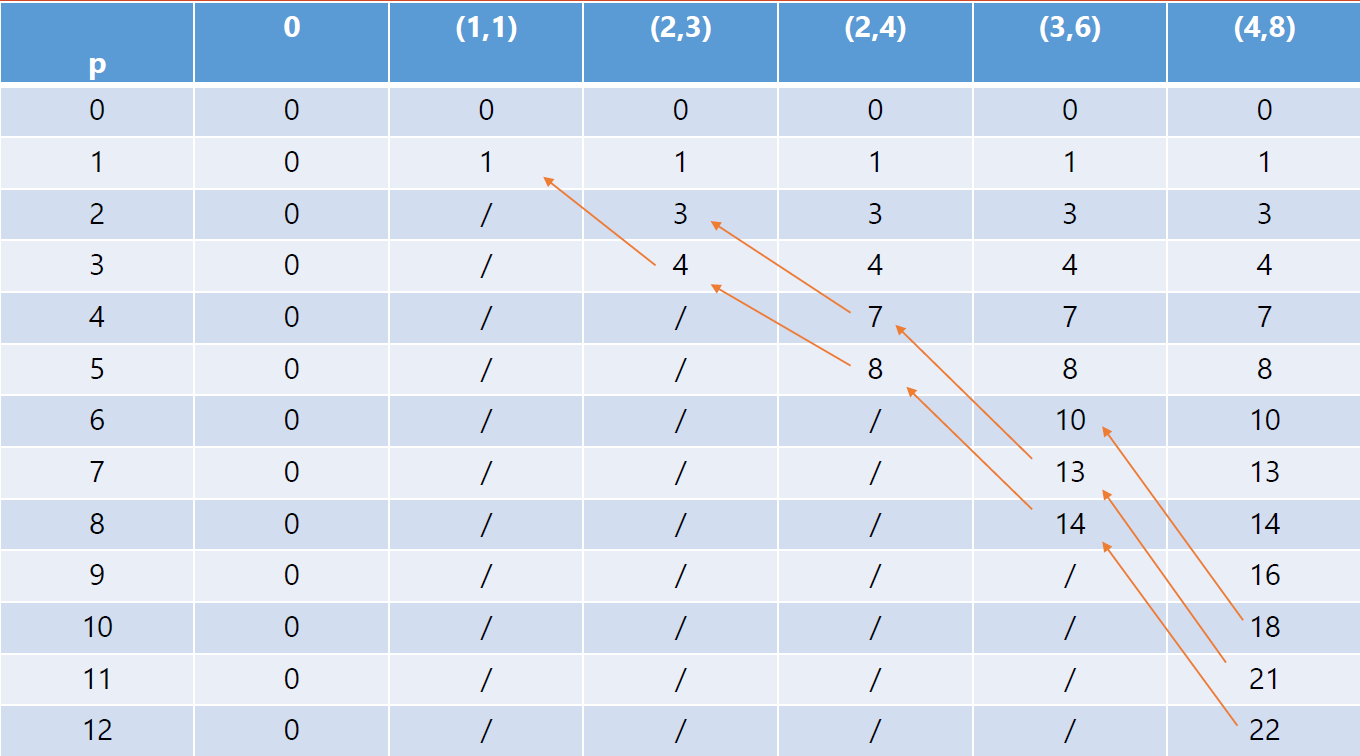
\includegraphics[width=\linewidth]{KnapsackDPAlgo2.png}
    \caption{Knapsack $\theta$(Vn) DP algorithm}
    \label{fig:Knapsack_example}
\end{figure}
\FloatBarrier

\subsection{Other examples of DP algorithms}

Before reading this section, please remember that all algorithm that can be
implemented via dynamic programming are not ipso-facto pseudo polynomial ! Any
algorithm can be expressed with dynamic programming as long as it can be separated in
sub problems.

\subsubsection{Edit distance}

TODO

\subsubsection{TSP}
 
TODO